\section{Experiment}
To verify the reliability of the water balance model for high-power fuel cell systems, it is necessary to record the water-containing state of the high-power fuel cell system when it reaches water balance under different operating conditions. Therefore, the experimental conditions should meet the following three points:(1) : The selected operating parameters should be within the normal operating range of the fuel cell system to avoid other faults in the fuel cell system other than water content faults (such as insufficient supply of reaction gas, air compressor surge, proportional valve failure, etc.), (2)In order to study the phenomena when the fuel cell system has a water content fault, the designed experiment needs to reflect more obvious phenomena under dry and flooded conditions, (3) The steady-state operation time should be long enough to ensure that the water content inside the fuel cell is in dynamic balance during this period, avoiding the impact of dynamic characteristics on the experimental results.
\subsection{Experiment Design}
The literature indicates that the factors that have the greatest impact on the water content inside the fuel cell are the air metering ratio, working temperature, and load current \cite{legrosFirstResultsPEMFC2011}. Since the temperature inside the stack cannot be measured during operation, the inlet temperature of the coolant is used as the working temperature in this paper, and the working temperature in the following text refers to the inlet temperature of the coolant. According to the operating conditions recommended by the system side, a three-factor five-level water content experiment was designed. The parameters of the experiment are shown in \ref{tab:WaterStateExperimentalParameterTable}.
\begin{table}
	\centering
	\begin{center}
		\caption{Water state experimental parameter table}
		\label{tab:WaterStateExperimentalParameterTable}
		\begin{tabular}{l|c|r}
			\hline
			\textbf{Load current/A/currency density/A·cm-2} & \textbf{Working temperature/℃} & \textbf{Air metering ratio} \\
			\hline
			120/0.4                                         & 55,60,65,70,73                 & 2,2.2,2.4,2.6,2.8           \\
			210/0.7                                         & 55,60,65,70,73                 & 1.8,2,2.2,2.4               \\
			300/1.0                                         & 63,65,68,70,73                 & 1.8,2,2.2,2.4               \\
			\hline
		\end{tabular}
	\end{center}
\end{table}

Literatures\cite{wuDiagnosticToolsPEM2008} indicates that the time required for the fuel cell system to reach water balance is generally a few seconds to ten minutes. Therefore, each test point ran for 20 minutes, and it was assumed that the fuel cell was in the process of establishing water balance within the first 15 minutes, and no data was recorded for this process, and the data obtained in the last 5 minutes was recorded. During the test, if a single cell voltage is too low or other faults cause the fuel cell system to shut down, the data of this operating point will be removed.


% 2.2章
\subsection{Test platform introduction}
The high-power fuel cell system used in this article is shown in Fig 2, manufactured by AT\&M Environmental Engineering Technology Co. The rated net output power of the fuel cell system is 100kW, the stack is composed of 410 single cells. High-pressure dry hydrogen gas enters the anode of the reaction stack after being depressurized by the solenoid valve and proportional valve. The liquid water in the residual hydrogen is separated by the gas-water separation device and intermittently discharged through the drain valve.
\begin{figure}[h]
	\centering
	\label{fig:PowerSystemDiagram}
	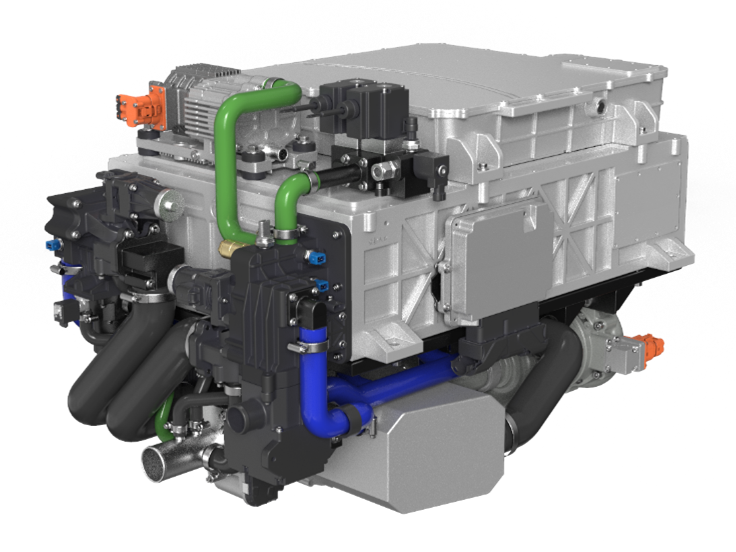
\includegraphics[scale=0.4]{Research_pictures/picture2.png}
	\caption[short]{power system diagram}
\end{figure}

For the above fuel cell system, the water balance model can be represented as
\begin{equation} \label{waterBalanceModel}
	\frac{d m_{w,s y s}}{d t}=Q_{v,i n,s y s}+Q_{w,g e n,c a}-Q_{w,o u t,c a}-Q_{w,o u t,a n}
\end{equation}

In formula (\ref{waterBalanceModel}), epresents the water
\begin{itemize}
	\item $m_(w,sys)$ represents the water content inside the fuel cell system, in grams.
	\item $Q_(v,in,sys)$ represents the flow rate of water vapor entering the fuel cell system, in g/s;
	\item $Q_(w,gen)$ represents the water flow generated by the electrochemical reaction, in g/s;
	\item $Q_(w,out,ca)$ represents the water flow out of the system from the air subsystem, in g/s;
	\item $Q_(w,out,an)$ represents the water flow out of the system from the hydrogen subsystem, in g/s;
\end{itemize}
Taking the fuel cell system during steady-state operation as the research object,
the change in the water content of the auxiliary system of the fuel cell system can be ignored, that is,
\begin{equation}\label{changeInWaterContent}
	\frac{d m_{w,s t k}}{d t}=\frac{d m_{w,s y s}}{d t}
\end{equation}
Each part of the equation can be calculated by:
\subsection*{Water flow into the system}
Since the hydrogen entering the system is high-pressure hydrogen with a purity of 99.99\%, water vapor mainly enters the system with the air. By recording the temperature, humidity, pressure of the environment during the reaction process, and the air flow entering the system, the water flow entering the system can be calculated.
\begin{equation}\label{waterFlowEnteringSystemCalculation}
	Q_{v,i n,s y s}={\frac{Q_{a i r;i n,s y s}\cdot P_{v a m b} \cdot M_{v}}{M_{a} \cdot P_{a m b}}}={\frac{Q_{a i r;i n,s y s}\cdot (P_{a m b} - P_{s a t} \ast RH)\cdot M_{v}}{M_{a} \cdot P_{a m b}}}
\end{equation}
In Formula(\ref{waterFlowEnteringSystemCalculation}),
\begin{itemize}
	\item $Q_{a i r;i n,s y s}$ stands for air flow into the system, in g/s;
	\item $P_{a m b}$ stands for environmental pressure, in kPa;
	\item $R_{v}$ represents the relative humidity of the environment;
	\item $P_{sat}$ represents the saturated vapor pressure of the environment, which can be calculated using the saturated water vapor pressure formula.
\end{itemize}

\begin{equation}
	p_{sat}\,= \exp \left(9.3876-{\frac{3826.36}{T_{a m b}-45.47}}\right)\times\,10^{3}
\end{equation}
\begin{itemize}
	\item $T_{amb}$ represents environmental temperature, K;
	\item $M_{v}$ represents water relative molecule mass, in g/mol;
	\item $M_{a}$ represents water relative molecule mass, in g/mol;
\end{itemize}
\subsection*{Water flow by electrochemical reaction}
The water flow produced by electrochemical reaction can be presented as formula below:
\begin{equation}
	Q_{v,g e n,c a}=\frac{{N\cdot M_{v}\cdot I_{s t}}}{2F}
\end{equation}
\begin{itemize}
	\item $N$ represents the number of single cells in the fuel cell stack.
	\item $I_{st}$ represents load current, in A.
	\item $F$ stands for faraday constant, which is 96485C/mol.
\end{itemize}
\subsection*{The water flow out of the system from the air side and the hydrogen side}
To measure the water flow out of the system from the air and hydrogen sides, this article has designed an exhaust water content detection device centered on condensation.
\begin{figure}
	\label{fig:water_detection_device_diagram}
	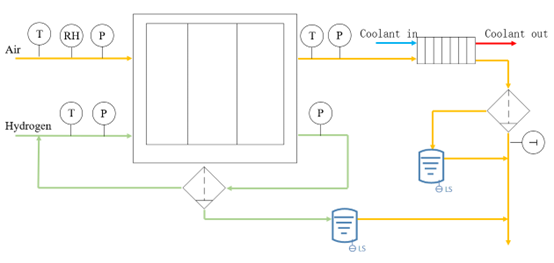
\includegraphics{Research_pictures/picture3.png}[scale=0.4]
	\caption[short]{Schematic diagram of exhaust gas water content detection device}
\end{figure}
The exhaust water content detection device on the air side is composed of a heat exchanger, a water separator, a temperature sensor, and a water collection device with a liquid level sensor. The basic principle is to condense the high-temperature supersaturated exhaust gas on the air side, and then separate the liquid water inside from the exhaust gas through the water separator, thus obtaining saturated low-temperature exhaust gas and liquid water. Collect the separated liquid water and collect the liquid level with a liquid level sensor.
Therefore, the water flow out of the system from the air side is composed of two parts: the liquid water collected in the air side collection device and the water vapor carried in the saturated steam after water vapor separation, that is,
\begin{equation}
	\label{waterFlowOutOfTheSystem}
	Q_{w,out,ca}={\frac{d m_{w,cacollect}}{d t}}+{\frac{Q_{air,out,sys} \cdot p_{v,sat}\cdot M_{v}}{M_{a} \cdot P_{a m b}}}
\end{equation}
In formula(\ref{waterFlowOutOfTheSystem}),
\begin{itemize}
	\item $m_{w,cacollect}$ represents the mass of the liquid collected by the exhaust water collection device on the air side, in grams(g);
	\item $Q_{air,out,sys}$ represents the air flow out of the system, in g(gram)/s(second), which can be calculated by the following formula.
\end{itemize}
The $Q_{air,out,sys}$ is represented as below:
\begin{equation}
	\label{airFlowOutOfTheSystem}
	Q_{air,outsys}=Q_{air,in,sys}-Q_{o,recat,ca}+Q_{v,gen,ca}-{\frac{dm_{w,cacolect}}{dt}}
\end{equation}
Since the hydrogen return circuit of the system is equipped with a water separator, the water content detection device on the hydrogen side mainly collects liquid water and a small amount of hydrogen, with less gaseous water, which does not significantly affect the experimental results. Therefore, the exhaust water content detection device on the hydrogen side only has a water collection device with a liquid level sensor, which is used to record the water flow discharged from the hydrogen side.
\begin{equation}
	Q_{w,out,an}={\frac{dm_{w,ancollect}}{dt}}
\end{equation}
$m_{w,ancollect}$ represents the mass of the liquid collected by the exhaust water collection device on the hydrogen side, in grams(g).

\subsection*{Test methods}
In sequence, turn on host computer, system controller, electronic load, auxiliary devices, and impedance testing system; Turn on the water pump, solenoid valve, proportional valve, back pressure valve, air compressor, drain valve, and hydrogen circulation pump in sequence, setting the anode inlet gas pressure 10kPa higher than the cathode inlet gas pressure ($\Delta p=20kPa$).
\par
Gradually load the system to 120A, adjust the speed of the air compressor and the opening angle of the back pressure valve, so that the air flow rate reaches the air metering coefficient of 2.8 corresponding to the target current, gradually raise the working temperature to 55±1℃, and start the temperature closed-loop control program to maintain this temperature; After the working temperature is stable at 55±1℃, start timing and run for a total of 15 minutes; Adjust the speed of the air compressor and the opening angle of the back pressure valve, so that the air metering ratio gradually decreases in the range of 2 ~2.8 with a step size of 0.2; Raise the working temperature to 60±1℃, 65±1℃, 70±1 , 73±1℃, repeat the testing phase and record the experimental data.
\par
Load up to 210A, 300A, repeat all recording steps, until all operating points water content detection experiments are completed.
\par
Gradually reduce the load to 0A, use nitrogen to purge the circuit, turn off the machine, and power down in sequence.